%%=============================================================================
%% LaTeX sjabloon voor bachelorproef, HoGent Bedrijf en Organisatie
%% Opleiding Toegepaste Informatica
%%=============================================================================

\documentclass[fleqn,a4paper,12pt]{book}

%%=============================================================================
%% LaTeX sjabloon voor de bachelorproef, HoGent Bedrijf en Organisatie
%% Opleiding toegepaste informatica
%%
%% Structuur en algemene vormgeving. Meestal hoef je hier niets te wijzigen.
%%
%% Vormgeving gebaseerd op "The Legrand Orange Book", version 2.0 (9/2/15)
%% door Mathias Legrand (legrand.mathias@gmail.com) met aanpassingen door
%% Vel (vel@latextemplates.com). Het oorspronkelijke template is te vinden op
%% http://www.LaTeXTemplates.com
%%
%% Aanpassingen voor HoGent toegepaste informatica: 
%%   Bert Van Vreckem <bert.vanvreckem@hogent.be>
%% Licentie: 
%%   CC BY-NC-SA 3.0 (http://creativecommons.org/licenses/by-nc-sa/3.0/)
%%=============================================================================

%%-----------------------------------------------------------------------------
%% Packages
%%-----------------------------------------------------------------------------

\usepackage[top=3cm,bottom=3cm,left=3cm,right=3cm,headsep=10pt,a4paper]{geometry} % Page margins
\usepackage[utf8]{inputenc}  % Accenten gebruiken in tekst (vb. é ipv \'e)
\usepackage{amsfonts}        % AMS math packages: extra wiskundige
\usepackage{amsmath}         %   symbolen (o.a. getallen-
\usepackage{amssymb}         %   verzamelingen N, R, Z, Q, etc.)
\usepackage[english,dutch]{babel}    % Taalinstellingen: woordsplitsingen,
                             %  commando's voor speciale karakters
                             %  ("dutch" voor NL)
                             

\usepackage{listings}
\usepackage{iflang}
\usepackage{eurosym}         % Euro-symbool €
\usepackage{geometry}
\usepackage{graphicx}        % Invoegen van tekeningen
\graphicspath{{img/}}       % Specifies the directory where pictures are stored
\usepackage{tikz}            % Required for drawing custom shapes
\usepackage[pdftex,bookmarks=true]{hyperref}
\usepackage{titlesec}
\usepackage[most]{tcolorbox}
                             % PDF krijgt klikbare links & verwijzingen,
                             %  inhoudstafel
\usepackage{enumitem}        % Customize lists
\setlist{nolistsep}         % Reduce spacing between list items
\usepackage{listings}        % Broncode mooi opmaken
\usepackage{multirow}        % Tekst over verschillende cellen in tabellen
\usepackage{rotating}        % Tabellen en figuren roteren

\usepackage{booktabs}        % Required for nicer horizontal rules in tables

\usepackage{xcolor}          % Required for specifying colors by name
\definecolor{maincolor}{RGB}{0,147,208} % Define the main color used for 
                             % highlighting throughout the book
                             % 0, 147, 208 = officiële kleur HoGent FBO
\newtcblisting{cisco}[1][]{size=fbox, listing only, listing options={style=tcblatex,basicstyle=\ttfamily\scriptsize,tabsize=2,language=sh},#1}

% Paragraph style: no indent, add space between paragraphs
\setlength{\parindent}{0em}
\setlength{\parskip}{1em}

\usepackage{etoolbox}
\usepackage{titling} % Macros for title, author, etc
\usepackage{lipsum}          % Voor vultekst (lorem ipsum)

%----------------------------------------------------------------------------------------
%	FONTS
%----------------------------------------------------------------------------------------

\usepackage{avant} % Use the Avantgarde font for headings
%\usepackage{times} % Use the Times font for headings
\usepackage{mathptmx} % Use the Adobe Times Roman as the default text font together with math symbols from the Sym­bol, Chancery and Com­puter Modern fonts

\usepackage{microtype} % Slightly tweak font spacing for aesthetics
\usepackage[utf8]{inputenc} % Required for including letters with accents
\usepackage[T1]{fontenc} % Use 8-bit encoding that has 256 glyphs

%------------------------------------------------------------------------------
%	TITLE PAGE
%------------------------------------------------------------------------------

\newcommand{\inserttitlepage}{%
\begin{titlepage}
  \newgeometry{top=2cm,bottom=1.5cm,left=1.5cm,right=1.5cm}
  \begin{center}

    \begingroup
    \rmfamily
    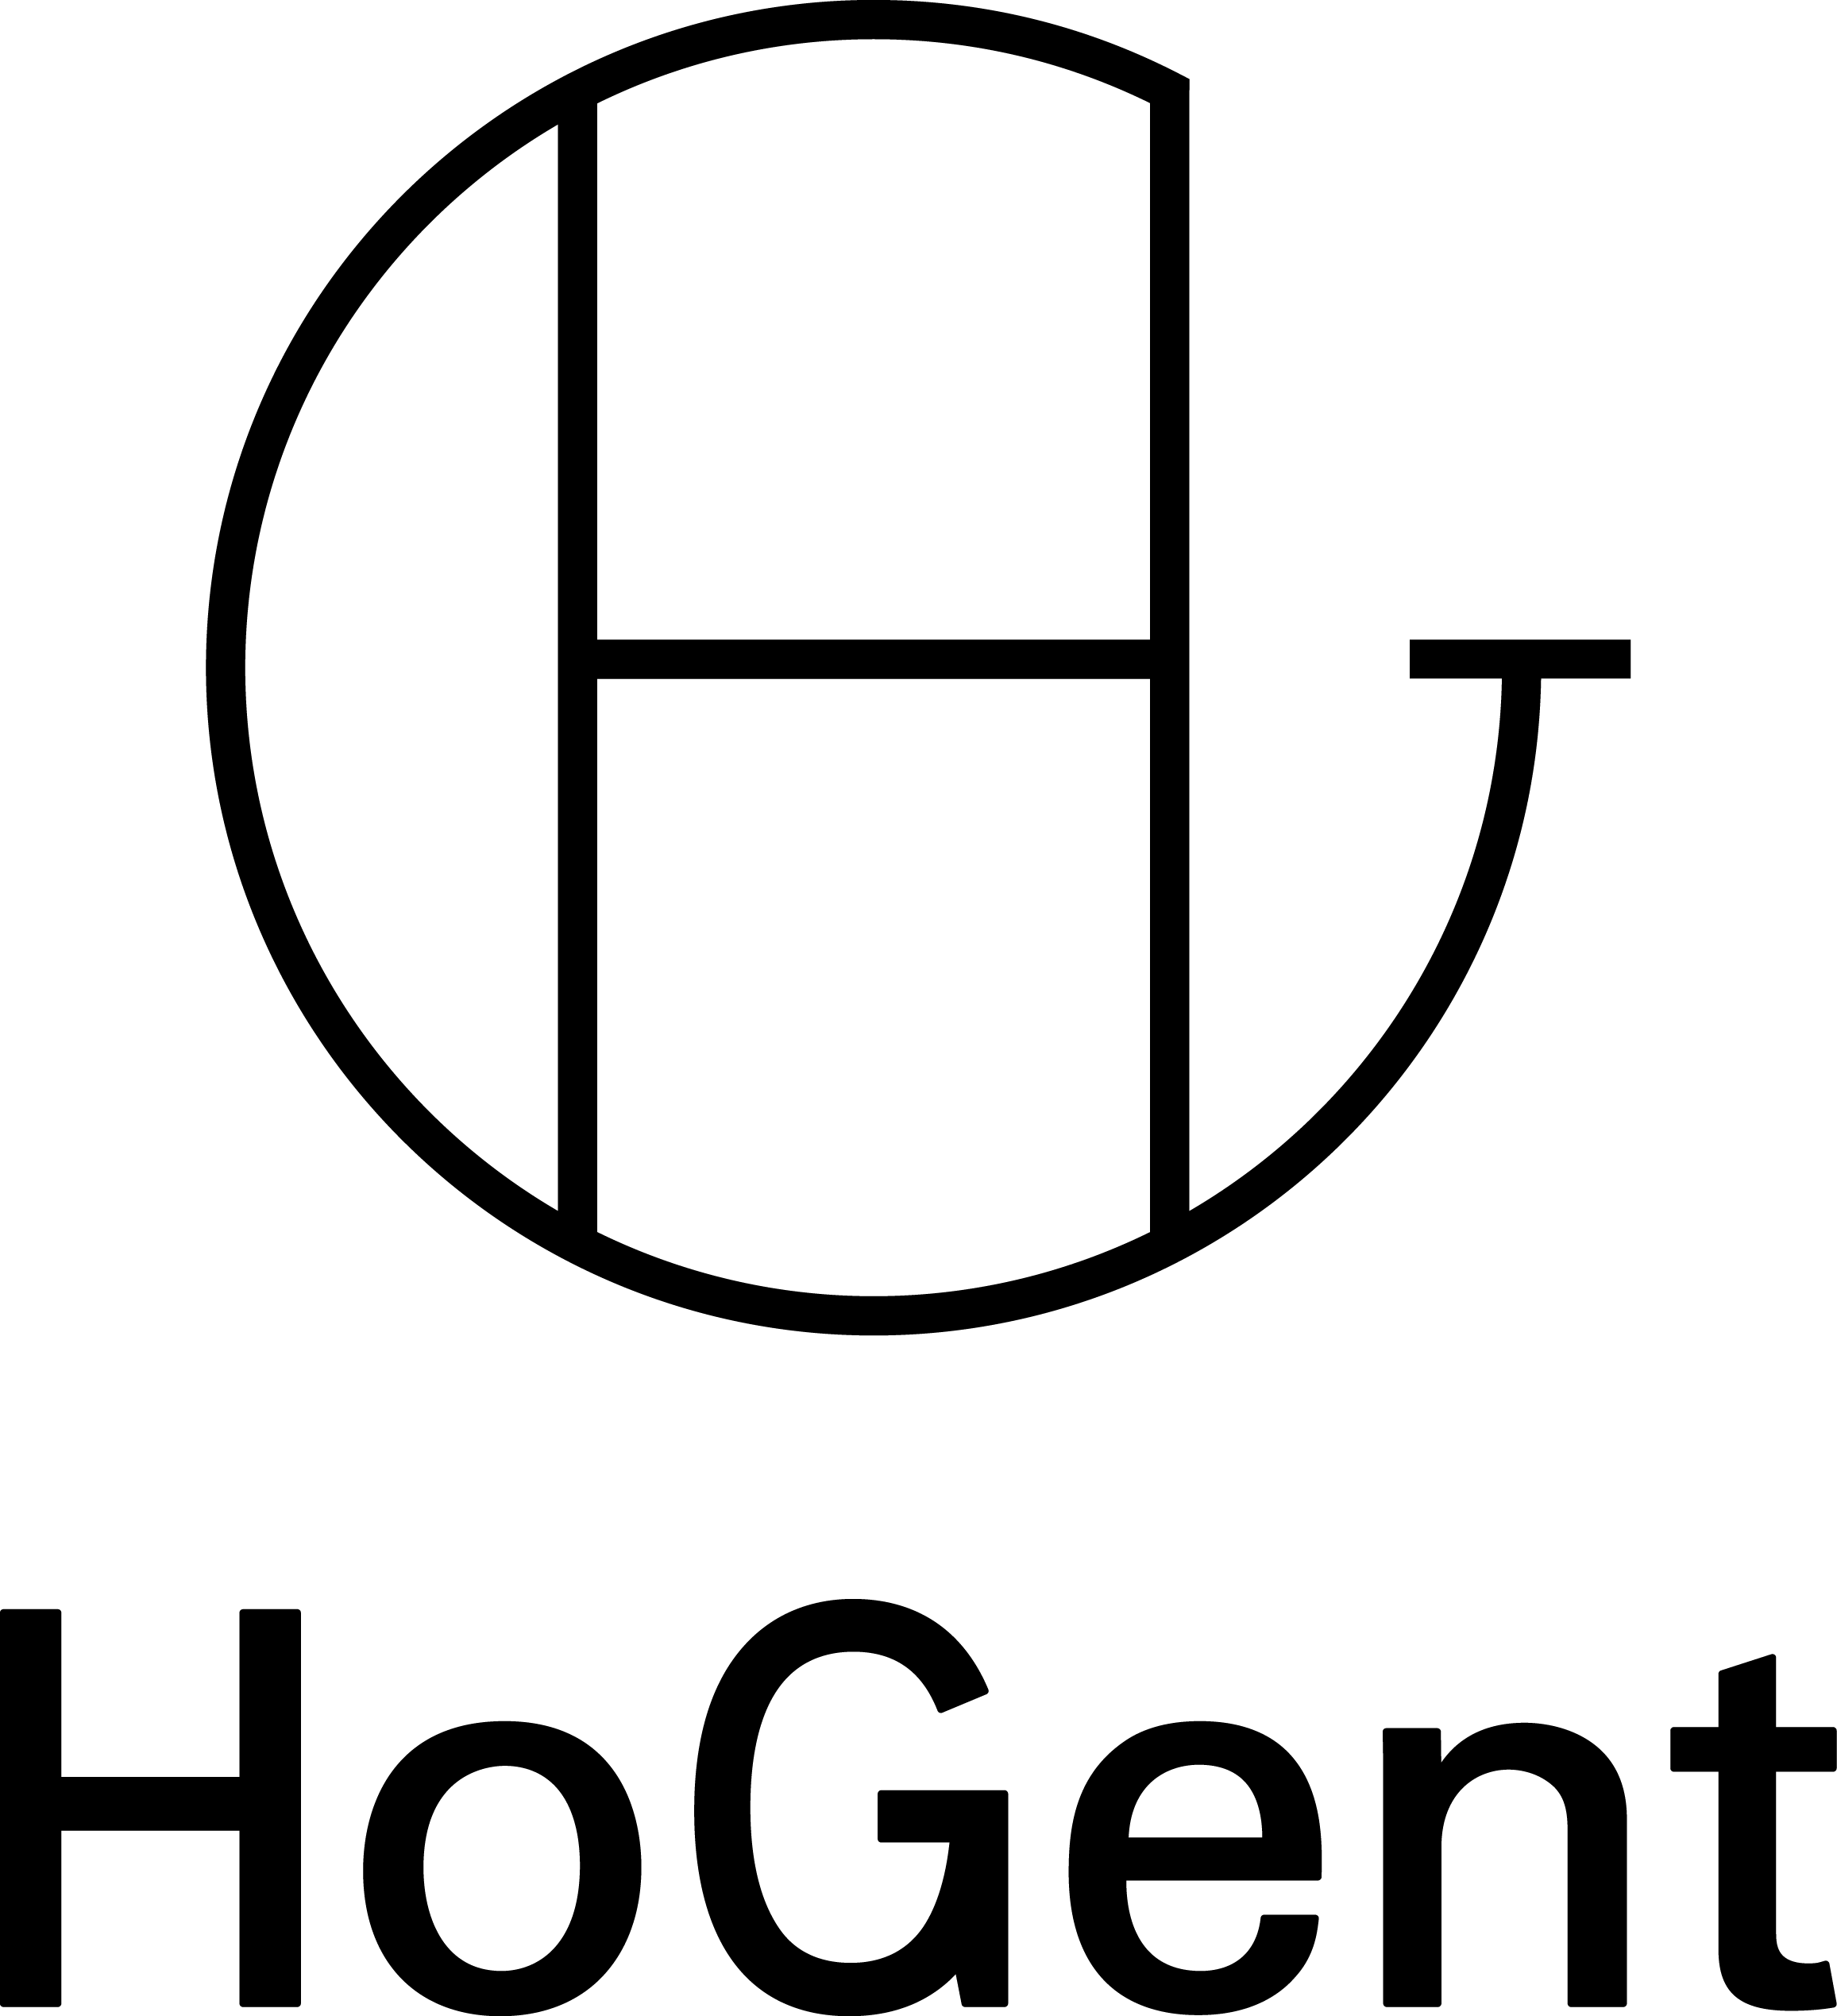
\includegraphics[width=2.5cm]{img/HG-beeldmerk-woordmerk}\\[.5cm]
    Faculteit Bedrijf en Organisatie\\[3cm]
    \titel
    \vfill
    \student\\[3.5cm]
    Scriptie voorgedragen tot het bekomen van de graad van\\professionele bachelor in de toegepaste informatica\\[2cm]
    Promotor:\\
    \promotor\\
    \ifdefempty{\copromotor}{\vspace{2.5cm}}{Co-promotor:\\\copromotor\\[2.5cm]}
    Instelling: \instelling\\[.5cm]
    Academiejaar: \academiejaar\\[.5cm]
    \ifcase \examenperiode \or Eerste \or Tweede \else Derde \fi examenperiode
    \endgroup

  \end{center}
  \restoregeometry
\end{titlepage}
  \emptypage
\begin{titlepage}
  \newgeometry{top=5.35cm,bottom=1.5cm,left=1.5cm,right=1.5cm}
  \begin{center}

    \begingroup
    \rmfamily
    \IfLanguageName{dutch}{Faculteit Bedrijf en Organisatie}{Faculty of Business and Information Management}\\[3cm]
    \titel
    \vfill
    \student\\[3.5cm]
    \IfLanguageName{dutch}{Scriptie voorgedragen tot het bekomen van de graad van\\professionele bachelor in de toegepaste informatica}{Thesis submitted in partial fulfilment of the requirements for the degree of\\professional bachelor of applied computer science}\\[2cm]
    Promotor:\\
    \promotor\\
    \ifdefempty{\copromotor}{\vspace{2.5cm}}{Co-promotor:\\\copromotor\\[2.5cm]}
    \IfLanguageName{dutch}{Instelling}{Institution}: \instelling\\[.5cm]
    \IfLanguageName{dutch}{Academiejaar}{Academic year}: \academiejaar\\[.5cm]
    \IfLanguageName{dutch}{%
    \ifcase \examenperiode \or Eerste \or Tweede \else Derde \fi examenperiode}{%
    \ifcase \examenperiode \or First \or Second \else Third \fi examination period}
    \endgroup

  \end{center}
  \restoregeometry
\end{titlepage}
}

%----------------------------------------------------------------------------------------
%	BIBLIOGRAPHY AND INDEX
%----------------------------------------------------------------------------------------

\usepackage[style=apa,backend=biber]{biblatex}
\usepackage{csquotes}
\DeclareLanguageMapping{dutch}{dutch-apa}
\addbibresource{bachproef-tin.bib} % BibTeX bibliography file
\addbibresource{../voorstel/voorstel.bib}
\defbibheading{bibempty}{}

\usepackage{calc} % For simpler calculation - used for spacing the index letter headings correctly
\usepackage{makeidx} % Required to make an index
\makeindex % Tells LaTeX to create the files required for indexing

%----------------------------------------------------------------------------------------
%	MAIN TABLE OF CONTENTS
%----------------------------------------------------------------------------------------

\usepackage{titletoc} % Required for manipulating the table of contents

\contentsmargin{0cm} % Removes the default margin

% Part text styling
\titlecontents{part}[0cm]
{\addvspace{20pt}\centering\large\bfseries}
{}
{}
{}

% Chapter text styling
\titlecontents{chapter}[1.25cm] % Indentation
{\addvspace{12pt}\large\sffamily\bfseries} % Spacing and font options for chapters
{\color{maincolor!60}\contentslabel[\Large\thecontentslabel]{1.25cm}\color{maincolor}} % Chapter number
{\color{maincolor}}
{\color{maincolor!60}\normalsize\;\titlerule*[.5pc]{.}\;\thecontentspage} % Page number

% Section text styling
\titlecontents{section}[1.25cm] % Indentation
{\addvspace{3pt}\sffamily\bfseries} % Spacing and font options for sections
{\contentslabel[\thecontentslabel]{1.25cm}} % Section number
{}
{\hfill\color{black}\thecontentspage} % Page number
[]

% Subsection text styling
\titlecontents{subsection}[1.25cm] % Indentation
{\addvspace{1pt}\sffamily\small} % Spacing and font options for subsections
{\contentslabel[\thecontentslabel]{1.25cm}} % Subsection number
{}
{\ \titlerule*[.5pc]{.}\;\thecontentspage} % Page number
[]

% List of figures
\titlecontents{figure}[0em]
{\addvspace{-5pt}\sffamily}
{\thecontentslabel\hspace*{1em}}
{}
{\ \titlerule*[.5pc]{.}\;\thecontentspage}
[]

% List of tables
\titlecontents{table}[0em]
{\addvspace{-5pt}\sffamily}
{\thecontentslabel\hspace*{1em}}
{}
{\ \titlerule*[.5pc]{.}\;\thecontentspage}
[]

%----------------------------------------------------------------------------------------
%	MINI TABLE OF CONTENTS IN PART HEADS
%----------------------------------------------------------------------------------------

% Chapter text styling
\titlecontents{lchapter}[0em] % Indenting
{\addvspace{15pt}\large\sffamily\bfseries} % Spacing and font options for chapters
{\color{maincolor}\contentslabel[\Large\thecontentslabel]{1.25cm}\color{maincolor}} % Chapter number
{}
{\color{maincolor}\normalsize\sffamily\bfseries\;\titlerule*[.5pc]{.}\;\thecontentspage} % Page number

% Section text styling
\titlecontents{lsection}[0em] % Indenting
{\sffamily\small} % Spacing and font options for sections
{\contentslabel[\thecontentslabel]{1.25cm}} % Section number
{}
{}

% Subsection text styling
\titlecontents{lsubsection}[.5em] % Indentation
{\normalfont\footnotesize\sffamily} % Font settings
{}
{}
{}

%----------------------------------------------------------------------------------------
%	PAGE HEADERS
%----------------------------------------------------------------------------------------

\usepackage{fancyhdr} % Required for header and footer configuration

\pagestyle{fancy}
\renewcommand{\chaptermark}[1]{\markboth{\sffamily\normalsize\bfseries\chaptername\ \thechapter.\ #1}{}} % Chapter text font settings
\renewcommand{\sectionmark}[1]{\markright{\sffamily\normalsize\thesection\hspace{5pt}#1}{}} % Section text font settings
\fancyhf{} \fancyhead[LE,RO]{\sffamily\normalsize\thepage} % Font setting for the page number in the header
\fancyhead[LO]{\rightmark} % Print the nearest section name on the left side of odd pages
\fancyhead[RE]{\leftmark} % Print the current chapter name on the right side of even pages
\renewcommand{\headrulewidth}{0.5pt} % Width of the rule under the header
\addtolength{\headheight}{2.5pt} % Increase the spacing around the header slightly
\renewcommand{\footrulewidth}{0pt} % Removes the rule in the footer
\fancypagestyle{plain}{\fancyhead{}\renewcommand{\headrulewidth}{0pt}} % Style for when a plain pagestyle is specified

% Removes the header from odd empty pages at the end of chapters
\makeatletter
\renewcommand{\cleardoublepage}{
\clearpage\ifodd\c@page\else
\hbox{}
\vspace*{\fill}
\thispagestyle{empty}
\newpage
\fi}

%----------------------------------------------------------------------------------------
%	THEOREM STYLES
%----------------------------------------------------------------------------------------

\usepackage{amsmath,amsfonts,amssymb,amsthm} % For math equations, theorems, symbols, etc

\newcommand{\intoo}[2]{\mathopen{]}#1\,;#2\mathclose{[}}
\newcommand{\ud}{\mathop{\mathrm{{}d}}\mathopen{}}
\newcommand{\intff}[2]{\mathopen{[}#1\,;#2\mathclose{]}}
\newtheorem{notation}{Notation}[chapter]

% Boxed/framed environments
\newtheoremstyle{maincolornumbox}% % Theorem style name
{0pt}% Space above
{0pt}% Space below
{\normalfont}% % Body font
{}% Indent amount
{\small\bf\sffamily\color{maincolor}}% % Theorem head font
{\;}% Punctuation after theorem head
{0.25em}% Space after theorem head
{\small\sffamily\color{maincolor}\thmname{#1}\nobreakspace\thmnumber{\@ifnotempty{#1}{}\@upn{#2}}% Theorem text (e.g. Theorem 2.1)
\thmnote{\nobreakspace\the\thm@notefont\sffamily\bfseries\color{black}---\nobreakspace#3.}} % Optional theorem note
\renewcommand{\qedsymbol}{$\blacksquare$}% Optional qed square

\newtheoremstyle{blacknumex}% Theorem style name
{5pt}% Space above
{5pt}% Space below
{\normalfont}% Body font
{} % Indent amount
{\small\bf\sffamily}% Theorem head font
{\;}% Punctuation after theorem head
{0.25em}% Space after theorem head
{\small\sffamily{\tiny\ensuremath{\blacksquare}}\nobreakspace\thmname{#1}\nobreakspace\thmnumber{\@ifnotempty{#1}{}\@upn{#2}}% Theorem text (e.g. Theorem 2.1)
\thmnote{\nobreakspace\the\thm@notefont\sffamily\bfseries---\nobreakspace#3.}}% Optional theorem note

\newtheoremstyle{blacknumbox} % Theorem style name
{0pt}% Space above
{0pt}% Space below
{\normalfont}% Body font
{}% Indent amount
{\small\bf\sffamily}% Theorem head font
{\;}% Punctuation after theorem head
{0.25em}% Space after theorem head
{\small\sffamily\thmname{#1}\nobreakspace\thmnumber{\@ifnotempty{#1}{}\@upn{#2}}% Theorem text (e.g. Theorem 2.1)
\thmnote{\nobreakspace\the\thm@notefont\sffamily\bfseries---\nobreakspace#3.}}% Optional theorem note

% Non-boxed/non-framed environments
\newtheoremstyle{maincolornum}% % Theorem style name
{5pt}% Space above
{5pt}% Space below
{\normalfont}% % Body font
{}% Indent amount
{\small\bf\sffamily\color{maincolor}}% % Theorem head font
{\;}% Punctuation after theorem head
{0.25em}% Space after theorem head
{\small\sffamily\color{maincolor}\thmname{#1}\nobreakspace\thmnumber{\@ifnotempty{#1}{}\@upn{#2}}% Theorem text (e.g. Theorem 2.1)
\thmnote{\nobreakspace\the\thm@notefont\sffamily\bfseries\color{black}---\nobreakspace#3.}} % Optional theorem note
\renewcommand{\qedsymbol}{$\blacksquare$}% Optional qed square
\makeatother

% Defines the theorem text style for each type of theorem to one of the three styles above
\newcounter{dummy}
\numberwithin{dummy}{section}
\theoremstyle{maincolornumbox}
\newtheorem{theoremeT}[dummy]{Theorem}
\newtheorem{problem}{Problem}[chapter]
\newtheorem{exerciseT}{Exercise}[chapter]
\theoremstyle{blacknumex}
\newtheorem{exampleT}{Example}[chapter]
\theoremstyle{blacknumbox}
\newtheorem{vocabulary}{Vocabulary}[chapter]
\newtheorem{definitionT}{Definition}[section]
\newtheorem{corollaryT}[dummy]{Corollary}
\theoremstyle{maincolornum}
\newtheorem{proposition}[dummy]{Proposition}

%----------------------------------------------------------------------------------------
%	DEFINITION OF COLORED BOXES
%----------------------------------------------------------------------------------------

\RequirePackage[framemethod=default]{mdframed} % Required for creating the theorem, definition, exercise and corollary boxes

% Theorem box
\newmdenv[skipabove=7pt,
skipbelow=7pt,
backgroundcolor=black!5,
linecolor=maincolor,
innerleftmargin=5pt,
innerrightmargin=5pt,
innertopmargin=5pt,
leftmargin=0cm,
rightmargin=0cm,
innerbottommargin=5pt]{tBox}

% Exercise box
\newmdenv[skipabove=7pt,
skipbelow=7pt,
rightline=false,
leftline=true,
topline=false,
bottomline=false,
backgroundcolor=maincolor!10,
linecolor=maincolor,
innerleftmargin=5pt,
innerrightmargin=5pt,
innertopmargin=5pt,
innerbottommargin=5pt,
leftmargin=0cm,
rightmargin=0cm,
linewidth=4pt]{eBox}

% Definition box
\newmdenv[skipabove=7pt,
skipbelow=7pt,
rightline=false,
leftline=true,
topline=false,
bottomline=false,
linecolor=maincolor,
innerleftmargin=5pt,
innerrightmargin=5pt,
innertopmargin=0pt,
leftmargin=0cm,
rightmargin=0cm,
linewidth=4pt,
innerbottommargin=0pt]{dBox}

% Corollary box
\newmdenv[skipabove=7pt,
skipbelow=7pt,
rightline=false,
leftline=true,
topline=false,
bottomline=false,
linecolor=gray,
backgroundcolor=black!5,
innerleftmargin=5pt,
innerrightmargin=5pt,
innertopmargin=5pt,
leftmargin=0cm,
rightmargin=0cm,
linewidth=4pt,
innerbottommargin=5pt]{cBox}

% Creates an environment for each type of theorem and assigns it a theorem text style from the "Theorem Styles" section above and a colored box from above
\newenvironment{theorem}{\begin{tBox}\begin{theoremeT}}{\end{theoremeT}\end{tBox}}
\newenvironment{exercise}{\begin{eBox}\begin{exerciseT}}{\hfill{\color{maincolor}\tiny\ensuremath{\blacksquare}}\end{exerciseT}\end{eBox}}
\newenvironment{definition}{\begin{dBox}\begin{definitionT}}{\end{definitionT}\end{dBox}}
\newenvironment{example}{\begin{exampleT}}{\hfill{\tiny\ensuremath{\blacksquare}}\end{exampleT}}
\newenvironment{corollary}{\begin{cBox}\begin{corollaryT}}{\end{corollaryT}\end{cBox}}

%----------------------------------------------------------------------------------------
%	REMARK ENVIRONMENT
%----------------------------------------------------------------------------------------

\newenvironment{remark}{\par\vspace{10pt}\small % Vertical white space above the remark and smaller font size
\begin{list}{}{
\leftmargin=35pt % Indentation on the left
\rightmargin=25pt}\item\ignorespaces % Indentation on the right
\makebox[-2.5pt]{\begin{tikzpicture}[overlay]
\node[draw=maincolor!60,line width=1pt,circle,fill=maincolor!25,font=\sffamily\bfseries,inner sep=2pt,outer sep=0pt] at (-15pt,0pt){\textcolor{maincolor}{R}};\end{tikzpicture}} % Orange R in a circle
\advance\baselineskip -1pt}{\end{list}\vskip5pt} % Tighter line spacing and white space after remark

%----------------------------------------------------------------------------------------
%	SECTION NUMBERING IN THE MARGIN
%----------------------------------------------------------------------------------------

\makeatletter
\renewcommand{\@seccntformat}[1]{\llap{\textcolor{maincolor}{\csname the#1\endcsname}\hspace{1em}}}
\renewcommand{\section}{\@startsection{section}{1}{\z@}
{-4ex \@plus -1ex \@minus -.4ex}
{1ex \@plus.2ex }
{\normalfont\large\sffamily\bfseries}}
\renewcommand{\subsection}{\@startsection {subsection}{2}{\z@}
{-3ex \@plus -0.1ex \@minus -.4ex}
{0.5ex \@plus.2ex }
{\normalfont\sffamily\bfseries}}
\renewcommand{\subsubsection}{\@startsection {subsubsection}{3}{\z@}
{-2ex \@plus -0.1ex \@minus -.2ex}
{.2ex \@plus.2ex }
{\normalfont\small\sffamily\bfseries}}
\renewcommand\paragraph{\@startsection{paragraph}{4}{\z@}
{-2ex \@plus-.2ex \@minus .2ex}
{.1ex}
{\normalfont\small\sffamily\bfseries}}

%----------------------------------------------------------------------------------------
%	PART HEADINGS
%----------------------------------------------------------------------------------------

% numbered part in the table of contents
\newcommand{\@mypartnumtocformat}[2]{%
\setlength\fboxsep{0pt}%
\noindent\colorbox{maincolor!20}{\strut\parbox[c][.7cm]{\ecart}{\color{maincolor!70}\Large\sffamily\bfseries\centering#1}}\hskip\esp\colorbox{maincolor!40}{\strut\parbox[c][.7cm]{\linewidth-\ecart-\esp}{\Large\sffamily\centering#2}}}%
%%%%%%%%%%%%%%%%%%%%%%%%%%%%%%%%%%
% unnumbered part in the table of contents
\newcommand{\@myparttocformat}[1]{%
\setlength\fboxsep{0pt}%
\noindent\colorbox{maincolor!40}{\strut\parbox[c][.7cm]{\linewidth}{\Large\sffamily\centering#1}}}%
%%%%%%%%%%%%%%%%%%%%%%%%%%%%%%%%%%
\newlength\esp
\setlength\esp{4pt}
\newlength\ecart
\setlength\ecart{1.2cm-\esp}
\newcommand{\thepartimage}{}%
\newcommand{\partimage}[1]{\renewcommand{\thepartimage}{#1}}%
\def\@part[#1]#2{%
\ifnum \c@secnumdepth >-2\relax%
\refstepcounter{part}%
\addcontentsline{toc}{part}{\texorpdfstring{\protect\@mypartnumtocformat{\thepart}{#1}}{\partname~\thepart\ ---\ #1}}
\else%
\addcontentsline{toc}{part}{\texorpdfstring{\protect\@myparttocformat{#1}}{#1}}%
\fi%
\startcontents%
\markboth{}{}%
{\thispagestyle{empty}%
\begin{tikzpicture}[remember picture,overlay]%
\node at (current page.north west){\begin{tikzpicture}[remember picture,overlay]%
\fill[maincolor!20](0cm,0cm) rectangle (\paperwidth,-\paperheight);
\node[anchor=north] at (4cm,-3.25cm){\color{maincolor!40}\fontsize{220}{100}\sffamily\bfseries\@Roman\c@part};
\node[anchor=south east] at (\paperwidth-1cm,-\paperheight+1cm){\parbox[t][][t]{8.5cm}{
\printcontents{l}{0}{\setcounter{tocdepth}{1}}%
}};
\node[anchor=north east] at (\paperwidth-1.5cm,-3.25cm){\parbox[t][][t]{15cm}{\strut\raggedleft\color{white}\fontsize{30}{30}\sffamily\bfseries#2}};
\end{tikzpicture}};
\end{tikzpicture}}%
\@endpart}
\def\@spart#1{%
\startcontents%
\phantomsection
{\thispagestyle{empty}%
\begin{tikzpicture}[remember picture,overlay]%
\node at (current page.north west){\begin{tikzpicture}[remember picture,overlay]%
\fill[maincolor!20](0cm,0cm) rectangle (\paperwidth,-\paperheight);
\node[anchor=north east] at (\paperwidth-1.5cm,-3.25cm){\parbox[t][][t]{15cm}{\strut\raggedleft\color{white}\fontsize{30}{30}\sffamily\bfseries#1}};
\end{tikzpicture}};
\end{tikzpicture}}
\addcontentsline{toc}{part}{\texorpdfstring{%
\setlength\fboxsep{0pt}%
\noindent\protect\colorbox{maincolor!40}{\strut\protect\parbox[c][.7cm]{\linewidth}{\Large\sffamily\protect\centering #1\quad\mbox{}}}}{#1}}%
\@endpart}
\def\@endpart{\vfil\newpage
\if@twoside
\if@openright
\null
\thispagestyle{empty}%
\newpage
\fi
\fi
\if@tempswa
\twocolumn
\fi}

%----------------------------------------------------------------------------------------
%	CHAPTER HEADINGS
%----------------------------------------------------------------------------------------

% A switch to conditionally include a picture, implemented by  Christian Hupfer
\newif\ifusechapterimage
\usechapterimagetrue
\newcommand{\thechapterimage}{}%
\newcommand{\chapterimage}[1]{\ifusechapterimage\renewcommand{\thechapterimage}{#1}\fi}%
\def\@makechapterhead#1{%
{\parindent \z@ \raggedright \normalfont
\ifnum \c@secnumdepth >\m@ne
\if@mainmatter
\begin{tikzpicture}[remember picture,overlay]
\node at (current page.north west)
{\begin{tikzpicture}[remember picture,overlay]
\node[anchor=north west,inner sep=0pt] at (0,0) {\ifusechapterimage\includegraphics[width=\paperwidth]{\thechapterimage}\fi};
\draw[anchor=west] (\Gm@lmargin,-9cm) node [line width=2pt,rounded corners=15pt,draw=maincolor,fill=white,fill opacity=0.5,inner sep=15pt]{\strut\makebox[22cm]{}};
\draw[anchor=west] (\Gm@lmargin+.3cm,-9cm) node {\huge\sffamily\bfseries\color{black}\thechapter. #1\strut};
\end{tikzpicture}};
\end{tikzpicture}
\else
\begin{tikzpicture}[remember picture,overlay]
\node at (current page.north west)
{\begin{tikzpicture}[remember picture,overlay]
\node[anchor=north west,inner sep=0pt] at (0,0) {\ifusechapterimage\includegraphics[width=\paperwidth]{\thechapterimage}\fi};
\draw[anchor=west] (\Gm@lmargin,-9cm) node [line width=2pt,rounded corners=15pt,draw=maincolor,fill=white,fill opacity=0.5,inner sep=15pt]{\strut\makebox[22cm]{}};
\draw[anchor=west] (\Gm@lmargin+.3cm,-9cm) node {\huge\sffamily\bfseries\color{black}#1\strut};
\end{tikzpicture}};
\end{tikzpicture}
\fi\fi\par\vspace*{270\p@}}}

%-------------------------------------------

\def\@makeschapterhead#1{%
\begin{tikzpicture}[remember picture,overlay]
\node at (current page.north west)
{\begin{tikzpicture}[remember picture,overlay]
\node[anchor=north west,inner sep=0pt] at (0,0) {\ifusechapterimage\includegraphics[width=\paperwidth]{\thechapterimage}\fi};
\draw[anchor=west] (\Gm@lmargin,-9cm) node [line width=2pt,rounded corners=15pt,draw=maincolor,fill=white,fill opacity=0.5,inner sep=15pt]{\strut\makebox[22cm]{}};
\draw[anchor=west] (\Gm@lmargin+.3cm,-9cm) node {\huge\sffamily\bfseries\color{black}#1\strut};
\end{tikzpicture}};
\end{tikzpicture}
\par\vspace*{270\p@}}
\makeatother

%----------------------------------------------------------------------------------------
%	HYPERLINKS IN THE DOCUMENTS
%----------------------------------------------------------------------------------------

\usepackage{hyperref}
\hypersetup{hidelinks,backref=true,pagebackref=true,hyperindex=true,colorlinks=false,breaklinks=true,urlcolor= maincolor,bookmarks=true,bookmarksopen=false,pdftitle={Title},pdfauthor={Author}}
\usepackage{bookmark}
\bookmarksetup{
open,
numbered,
addtohook={%
\ifnum\bookmarkget{level}=0 % chapter
\bookmarksetup{bold}%
\fi
\ifnum\bookmarkget{level}=-1 % part
\bookmarksetup{color=maincolor,bold}%
\fi
}
}

%----------------------------------------------------------------------------------------
%	Java source code
%----------------------------------------------------------------------------------------

% Commando voor invoegen Java-broncodebestanden (dank aan Niels Corneille)
% Gebruik:
%   \codefragment{source/MijnKlasse.java}{Uitleg bij de code}
%
% Je kan dit aanpassen aan de taal die je zelf het meeste gebruikt in je
% bachelorproef.
\newcommand{\codefragment}[2]{ \lstset{%
  language=java,
  breaklines=true,
  float=th,
  caption={#2},
  basicstyle=\scriptsize,
  frame=single,
  extendedchars=\true
}
\lstinputlisting{#1}}

% Leeg blad
\newcommand{\emptypage}{%
\newpage
\thispagestyle{empty}
\mbox{}
\newpage
}


%%---------- Documenteigenschappen --------------------------------------------
%% TODO: Vul dit aan met je eigen info:

% Je eigen naam
\newcommand{\student}{Kjell Viaene}

% De naam van je promotor (lector van de opleiding)
\newcommand{\promotor}{Mevr. Margot De Donder}

% De naam van je co-promotor. Als je promotor ook je opdrachtgever is en je
% dus ook inhoudelijk begeleidt (en enkel dan!), mag je dit leeg laten.
\newcommand{\copromotor}{Dhr. Bert Van Vreckem}

% Indien je bachelorproef in opdracht van/in samenwerking met een bedrijf of
% externe organisatie geschreven is, geef je hier de naam. Zoniet laat je dit
% zoals het is.
\newcommand{\instelling}{---}

% De titel van het rapport/bachelorproef
\newcommand{\titel}{A secure environment for conducting examinations on personal devices}

% Datum van indienen (gebruik telkens de deadline, ook al geef je eerder af)
\newcommand{\datum}{27 may 2018}

% Academiejaar
\newcommand{\academiejaar}{2017-2018}

% Examenperiode
%  - 1e semester = 1e examenperiode => 1
%  - 2e semester = 2e examenperiode => 2
%  - tweede zit  = 3e examenperiode => 3
\newcommand{\examenperiode}{2}

%%=============================================================================
%% Inhoud document
%%=============================================================================

\begin{document}

%---------- Taalselectie ------------------------------------------------------
% Als je je bachelorproef in het Engels schrijft, haal dan onderstaande regel
% uit commentaar. Let op: de tekst op de voorkaft blijft in het Nederlands, en
% dat is ook de bedoeling!

\selectlanguage{english}

%---------- Titelblad ---------------------------------------------------------
\inserttitlepage

%---------- Samenvatting, voorwoord -------------------------------------------
\usechapterimagefalse
%%=============================================================================
%% Voorwoord
%%=============================================================================

\chapter*{Preface}
\label{ch:voorwoord}

%% TODO:
%% Het voorwoord is het enige deel van de bachelorproef waar je vanuit je
%% eigen standpunt (``ik-vorm'') mag schrijven. Je kan hier bv. motiveren
%% waarom jij het onderwerp wil bespreken.
%% Vergeet ook niet te bedanken wie je geholpen/gesteund/... heeft

This bachelor thesis was written as part of the course which shares the same name. This thesis together with the internship I'm currently doing are the final two courses to complete a bachelor diploma in Applied Informatics.
\section*{Choosing the subject}
The subject of the thesis is one I picked from a list of suggestions that were posted online on the school platform \textit{Chamillo}. The subject caught my eye because of my personal experience with the issue. There would be times were we would take digital examinations for certain courses and people all around me were cheating to get great results. I always found it rather disrespectful and disturbing that people were doing this and that they were able to this so easily. This is a real demotivation for students who actually study for the examinations. Because when you get the results and realize that everybody who cheats got better results than you, then why bother if no penalty are given out anyway.\\
This of course devalues the examination itself and the course as a whole. Resulting in people not taking courses with digital exams seriously and getting high grades without ever understanding what the course matter was really about.\\
So when the opportunity was there for me to possibly change this and help the school with solving the problem, I eagerly picked this as my subject for my bachelor thesis.
%%=============================================================================
%% Samenvatting
%%=============================================================================

% TODO: De "abstract" of samenvatting is een kernachtige (~ 1 blz. voor een
% thesis) synthese van het document.
%
% Deze aspecten moeten zeker aan bod komen:
% - Context: waarom is dit werk belangrijk?
% - Nood: waarom moest dit onderzocht worden?
% - Taak: wat heb je precies gedaan?
% - Object: wat staat in dit document geschreven?
% - Resultaat: wat was het resultaat?
% - Conclusie: wat is/zijn de belangrijkste conclusie(s)?
% - Perspectief: blijven er nog vragen open die in de toekomst nog kunnen
%    onderzocht worden? Wat is een mogelijk vervolg voor jouw onderzoek?
%
% LET OP! Een samenvatting is GEEN voorwoord!

%%---------- Nederlandse samenvatting -----------------------------------------
%
% TODO: Als je je bachelorproef in het Engels schrijft, moet je eerst een
% Nederlandse samenvatting invoegen. Haal daarvoor onderstaande code uit
% commentaar.
% Wie zijn bachelorproef in het Nederlands schrijft, kan dit negeren, de inhoud
% wordt niet in het document ingevoegd.

\IfLanguageName{english}{%
\selectlanguage{english}

\chapter*{Samenvatting (dutch)}
\selectlanguage{english}
}{ }
Het opzetten van een beveiligde digitale omgeving is altijd een uitdaging, ongeacht de situatie. Door de continue ontwikkeling van technologie, en zeker in het vakgebied van de informatica, is het soms uitdagend om de beveiliging even snel te doen mee evolueren. De kern van deze bachelor proef is het opzetten van een omgeving waarin studenten een digitaal examen kunnen afleggen in een omgeving waar de toegang tot bepaalde middelen zijn beperkt. Zodanig de kans op spieken verminderd. Een dergelijke omgeving is cruciaal bij het bepalen van de resultaten van testen en examens. Als studenten namelijk in staat zijn van eenvoudig te spieken tijdens een examen of test dan verliezen deze hun waarde in het vak. En zo zal er dan geen duidelijke weerspiegeling gevormd worden van hun kennis.
De school zelf zal zo onder de indruk zijn dat het vak te gemakkelijk is of niet waardevol is voor het grootste deel van de studenten. Hierdoor zal het vak misschien als minderwaardig worden gezien en zo ook de stof die in het vak wordt geleerd. Ook de studenten zelf zullen denken dat ze het vak onder de knie hebben en slagen voor hun examens. Echter zonder een doorgronde kennis van de stof, en dit zou later wel eens voor problemen kunnen zorgen. \\
Om zo een systeem op te zetten werd onderzoek gedaan naar verschillende mogelijke manieren voor het opzetten van een beveiligde netwerk omgeving voor het afleggen van digitale examens. Deze zijn:
\begin{itemize}
\item Het filteren op basis van een DNS Whitelist
\item Het filteren op basis van een ACL op een router
\item Het filteren op basis van een firewall
\item Het filteren a.d.h.v. een applicatie
\end{itemize}
Deze zijn de meest voor de hand liggende methoden die gebruikt worden om informatie te filteren in het netwerk. Er wordt onderzocht welke van deze methoden goed zijn en hoe goed ze zijn in wat ze doen. Ook de eenvoud van het configureren en kost wordt in rekening gebracht. \\
Na het testen van deze methoden kunnen we concluderen dat DNS whitelisting te veel werk vereist en te gemakkelijk omzeilt kan worden. ACL en een firewall hebben dit minder en zijn daarom betere keuzes. Echter het gebruik maken van een applicatie die lokaal op elke computer staat geïnstalleerd is de beste keuze die kan gemaakt worden. We spreken hier van Safe Exam Browser (SEB) wat werd vermeld in een thesis in de literatuurstudie en bleek een uitstekende tool te zijn om te gebruiken in deze probleemstelling. Het bereikt alle gewenste factoren en is gemakkelijk in het gebruik. Er is echter wel een nadeel, de tool is niet geïntegreerd met chamillo. Dit zou echter een onderwerp kunnen zijn voor verder onderzoek.



%%---------- Samenvatting -----------------------------------------------------
% De samenvatting in de hoofdtaal van het document

\chapter*{\IfLanguageName{english}{Summary}{Abstract}}
Setting up a secure environment in any situation is a challenge. With technology constantly evolving, especially in the IT sector, it's always hard to keep security up to date as well. The core of  the purpose in this thesis is to build a system that ensures students who are taking part in an examination only have access to those resources which they are allowed to use. \\ Having a system like this is crucial to having a good grading of courses. When students are able to cheat at examinations as easily as they often can now, all the value of an examination is lost.\\ For the school itself it would seem like the course is too easy and needs to be made harder. Which devalues the material that is being taught in this course.  \\
The students will think that they are having it easy and will pass the exam without any real knowledge of the subject. This may come back in later situations (follow up courses, job interviews, ...) where they then realize that they seem to be missing some knowledge that they were supposed to have.\\
Multiple methods were tested to find a system in which these problems are resolved. These methods are:
\begin{itemize}
\item Filtering using a DNS Whitelist
\item Filtering using an ACL on a router
\item Filtering using a firewall
\item Filtering using an application.
\end{itemize}
These are the most common ways of filtering internet access in a network. Research is done as to what method is good and how good these methods are compared with each other. How complicated they are to set up and maintain. After testing these methods a conclusion was made that DNS whitelisting is the worst choice. This methods requires the most work and performs the lowest. While the ACL on a router and a firewall are pretty even. They are easy to configure and allow for better protection. The firewall has more possibilities but can be harder to set up while the router is a bit simpler but is easy to set up. The best choice however is without a doubt the application (Safe Exam Browser). This application secures every device on its own and allows for local filtering of the internet and the local files. This is the perfect solution to our issue. It's easy to use and performs really well. The only downside to it is that there is no integration with Chamillo. It can still be used but some authorization methods are not applicable. This however could be the subject of an other research paper.

%---------- Inhoudstafel ------------------------------------------------------
\pagestyle{empty} % No headers
\tableofcontents % Print the table of contents itself
\cleardoublepage % Forces the first chapter to start on an odd page so it's on the right
\pagestyle{fancy} % Print headers again

%---------- Lijst figuren, afkortingen, ... -----------------------------------

% Indien gewenst kan je hier een lijst van figuren/tabellen opgeven. Geef in
% dat geval je figuren/tabellen altijd een korte beschrijving:
%
%  \caption[korte beschrijving]{uitgebreide beschrijving}

\listoffigures
\listoftables

% Als je een lijst van afkortingen of termen wil toevoegen, dan hoort die
% hier thuis. Gebruik bijvoorbeeld de ``glossaries'' package.
% https://www.sharelatex.com/learn/Glossaries

%%---------- Kern -------------------------------------------------------------

%%=============================================================================
%% Inleiding
%%=============================================================================

\chapter*{Inleiding}
\label{ch:inleiding}

De inleiding moet de lezer net genoeg informatie verschaffen om het onderwerp te begrijpen en in te zien waarom de onderzoeksvraag de moeite waard is om te onderzoeken. In de inleiding ga je literatuurverwijzingen beperken, zodat de tekst vlot leesbaar blijft. Je kan de inleiding verder onderverdelen in secties als dit de tekst verduidelijkt. Zaken die aan bod kunnen komen in de inleiding~\autocite{Pollefliet2011}:

\begin{itemize}
  \item context, achtergrond
  \item afbakenen van het onderwerp
  \item verantwoording van het onderwerp, methodologie
  \item probleemstelling
  \item onderzoeksdoelstelling
  \item onderzoeksvraag
  \item \ldots
\end{itemize}

\section{Probleemstelling}
\label{sec:probleemstelling}

Uit je probleemstelling moet duidelijk zijn dat je onderzoek een meerwaarde heeft voor een concrete doelgroep. De doelgroep moet goed gedefinieerd en afgelijnd zijn. Doelgroepen als ``bedrijven,'' ``KMO's,'' systeembeheerders, enz.~zijn nog te vaag. Als je een lijstje kan maken van de personen/organisaties die een meerwaarde zullen vinden in deze bachelorproef (dit is eigenlijk je steekproefkader), dan is dat een indicatie dat de doelgroep goed gedefinieerd is. Dit kan een enkel bedrijf zijn of zelfs één persoon (je co-promotor/opdrachtgever).

\section{Onderzoeksvraag}
\label{sec:onderzoeksvraag}

Wees zo concreet mogelijk bij het formuleren van je onderzoeksvraag. Een onderzoeksvraag is trouwens iets waar nog niemand op dit moment een antwoord heeft (voor zover je kan nagaan). Het opzoeken van bestaande informatie (bv. ``welke tools bestaan er voor deze toepassing?'') is dus geen onderzoeksvraag. Je kan de onderzoeksvraag verder specifiëren in deelvragen. Bv.~als je onderzoek gaat over performantiemetingen, dan 

\section{Onderzoeksdoelstelling}
\label{sec:onderzoeksdoelstelling}

Wat is het beoogde resultaat van je bachelorproef? Wat zijn de criteria voor succes? Beschrijf die zo concreet mogelijk.

\section{Opzet van deze bachelorproef}
\label{sec:opzet-bachelorproef}

% Het is gebruikelijk aan het einde van de inleiding een overzicht te
% geven van de opbouw van de rest van de tekst. Deze sectie bevat al een aanzet
% die je kan aanvullen/aanpassen in functie van je eigen tekst.

De rest van deze bachelorproef is als volgt opgebouwd:

In Hoofdstuk~\ref{ch:stand-van-zaken} wordt een overzicht gegeven van de stand van zaken binnen het onderzoeksdomein, op basis van een literatuurstudie.

In Hoofdstuk~\ref{ch:methodologie} wordt de methodologie toegelicht en worden de gebruikte onderzoekstechnieken besproken om een antwoord te kunnen formuleren op de onderzoeksvragen.

% TODO: Vul hier aan voor je eigen hoofstukken, één of twee zinnen per hoofdstuk

In Hoofdstuk~\ref{ch:conclusie}, tenslotte, wordt de conclusie gegeven en een antwoord geformuleerd op de onderzoeksvragen. Daarbij wordt ook een aanzet gegeven voor toekomstig onderzoek binnen dit domein.


\chapter{Stand van zaken}
\label{ch:stand-van-zaken}

% Tip: Begin elk hoofdstuk met een paragraaf inleiding die beschrijft hoe
% dit hoofdstuk past binnen het geheel van de bachelorproef. Geef in het
% bijzonder aan wat de link is met het vorige en volgende hoofdstuk.

% Pas na deze inleidende paragraaf komt de eerste sectiehoofding.

Dit hoofdstuk bevat je literatuurstudie. De inhoud gaat verder op de inleiding, maar zal het onderwerp van de bachelorproef *diepgaand* uitspitten. De bedoeling is dat de lezer na lezing van dit hoofdstuk helemaal op de hoogte is van de huidige stand van zaken (state-of-the-art) in het onderzoeksdomein. Iemand die niet vertrouwd is met het onderwerp, weet er nu voldoende om de rest van het verhaal te kunnen volgen, zonder dat die er nog andere informatie moet over opzoeken \autocite{Pollefliet2011}.

Je verwijst bij elke bewering die je doet, vakterm die je introduceert, enz. naar je bronnen. In \LaTeX{} kan dat met het commando \texttt{$\backslash${textcite\{\}}} of \texttt{$\backslash${autocite\{\}}}. Als argument van het commando geef je de ``sleutel'' van een ``record'' in een bibliografische databank in het Bib\TeX{}-formaat (een tekstbestand). Als je expliciet naar de auteur verwijst in de zin, gebruik je \texttt{$\backslash${}textcite\{\}}.
Soms wil je de auteur niet expliciet vernoemen, dan gebruik je \texttt{$\backslash${}autocite\{\}}. In de volgende paragraaf een voorbeeld van elk.

\textcite{Knuth1998} schreef een van de standaardwerken over sorteer- en zoekalgoritmen. Experten zijn het erover eens dat cloud computing een interessante opportuniteit vormen, zowel voor gebruikers als voor dienstverleners op vlak van informatietechnologie~\autocite{Creeger2009}.

\lipsum[7-20]

%%=============================================================================
%% Methodologie
%%=============================================================================

\chapter{Methodology}
\label{ch:methodologie}

To test the possible methods described earlier a virtual network was set up using Oracle VirtualBox \footnote{ https://www.virtualbox.org/} in combination with Vagrant \footnote{https://www.vagrantup.com/} and Ansible \footnote{https://www.ansible.com/}. The specifics of this test environment can be found in the next chapter. A physical network was not possible as this required to much materials and cost. The school is located to far as well to be able to build an environment there. Which resulted in the need of a virtual network. The only issue with the virtual network is the fact that only a computer with eight gigabytes of RAM is available, which sometimes is not that much when running four to five virtual machines.\\

For each method adjustments are made to the test environment. These adjustments already form a base to the conclusion made in the thesis as the difficulty of configuring the devices is a factor for evaluation. When the configurations have been completed it is tested if the wanted results have been reached. If this is the case, or if not, than a conclusion is made about the effectiveness of the method. In the final conclusion a bigger conclusion about all methods will be made based on these setups. Some loopholes and such that might have been encountered during the setups of these environments will be mentioned there as well.\\



















% Voeg hier je eigen hoofdstukken toe die de ``corpus'' van je bachelorproef
% vormen. De structuur en titels hangen af van je eigen onderzoek. Je kan bv.
% elke fase in je onderzoek in een apart hoofdstuk bespreken.

%\input{...}
%\input{...}
%...

%%=============================================================================
%% Conclusie
%%=============================================================================

\chapter{Conclusion}
\label{ch:conclusie}

%% TODO: Trek een duidelijke conclusie, in de vorm van een antwoord op de
%% onderzoeksvra(a)g(en). Wat was jouw bijdrage aan het onderzoeksdomein en
%% hoe biedt dit meerwaarde aan het vakgebied/doelgroep? Reflecteer kritisch
%% over het resultaat. Had je deze uitkomst verwacht? Zijn er zaken die nog
%% niet duidelijk zijn? Heeft het onderzoek geleid tot nieuwe vragen die
%% uitnodigen tot verder onderzoek?

\section{Comparing the different methods}
The obivous winner of these methods is SEB. It is extremely easy to implement, blocks traffic on way more levels than the other methods do and is very user friendly. And with the correct handling it could be quite unbreakable for students. It is amazing that a tool like this is not being used more frequently. The biggest reason for this is probably because a lot of people simply do not know that it exists. But as big contributors to this software are mostly located in countries who are leading in education worldwide it might not be a bad idea to pick this up.
Upon discovery of this tool the other methods kind off faded in importance and usefulness. As all the other methods only really tackle one issue in the wide range of cheating possibilities. But from the other tested methods DNS whitelisting seems to be the worst one. It has the most loopholes and is harder to implement than the other two are. As well as it has a bigger impact on the network. If a local DNS is already present there will have to be made quite some changes to the configuration. As well as the difficulty  of adding all the IP's and domain names to list. One might argue that a blacklist might be better because there are often offered online. But these will always be one step behind. It's easier to find a certain fish in a lake when only 6 fish are swimming in it, than it is in an ocean where millions of fish are swimming even though a few million have already been pulled out.\\
The ACL's and the firewall are on the same level. If one of these two would be chosen, it's really a matter of preference. The firewall allow for great configuration that goes way farther than simply filtering traffic. But it is once again an extra device that is needed. While a router is present in the network and can do the same functions that are required without having to spend anything new on equipment.  Plus in this thesis the configuration of the router went a lot smoother than the firewall. This can of course depend from system to system, which is way the choice between these really depends on the situation one is in. Both get the job done though. They are a lot easier to implement than DNS whitelisting is. They are more tightly sealed and are more difficult to trick.\\
So all around SEB is the overall winner with ACL's and firewall on a shared second place. A combination of the both could be used as well of course. When certain exams require specific multiple websites to be accessible SEB could be used to prevent the student from using any local documentation while an ACL could block the websites that are not allowed. Doing this one creates a flexible,dynamic and multi functional network in which exams can be made safely.
\section{Issues with the tested methods}
The biggest issue was the fact that a lot of these methods count on the IP or the full qualified domain name of a website. While this is not always as easy to get. A lot of (probably almost all) websites these days using multiple third party components to host their site. This means that simply allowing or blocking one IP-Address / FQDN does not do the trick. When we want to allow a website it might nog load completely or just refuse to load because of certain rules. And when blocking one it might still be accessible to some extend. Figuring out all the information needed to allow one website can be a lot of work and cause a lot of headaches. Furthermore, when the required information is found it might lead to a server on which multiple websites are stored. Trying to block that one website can be very irritating as these websites might change IP's which would lead to us blocking and allowing the wrong sites. Which of course is not in our interest.\\
An other exploit that might come to mind is the use of VPN's. These however could be blocked by blocking certain ports using a firewall/ACL's (which gives these an other advantage above DNS whitelisting). These ports might be quite big in numbers. But they could all be added to a single port group and then added to the block list whenever an exam is conducted. This way no VPN's would be possible but some other functions might malfunction as well at the same time (for some VPN systems for instance once would have to block the SSH port).\\
The last small issue is the fact that Chamillo was not a LSM that is integrated with SEB which limited the testing possibilities. Even though the system is pretty great with a not integrated LSM, it's always good to improve. Maybe someday the Chamillo community will take a look at this and integrate SEB.
\section{Concerns outside of the general environment}
A brief mention should be made to remind people that all the above methods can be made obsolete by some stupid mistakes. If a student manages to use his smartphone all walls are down again. The same goes with god old fashioned cheating using pen and paper. These systems should of course still be prevented by for instance collecting the phones at the start of an examination and handing them back after it. And using only see through pen cases or no pen cases at all. Equally harmful would be an uninformed teacher/overseer. If a student would be able to trick a teacher into giving them information that he should not know, just because the teacher is not someone with great IT knowledge, the whole system once again topples over. To prevent this all teachers and overseers should always be told the information they need. And to not share this information with anyone. Or call someone with the required knowledge when a problem occurs.
\section{Answering the research questions}
\subsubsection{Can we limit access to the internet to only the necessary item?}
A question that is not easily answered. But after this thesis the answer would be yes. Even though students will probably always find a way to circumvent the systems. At the time of deployment there is a possibility to make environments in which only access is given to the required resources. This can be done by using SEB, or ACL's or a combination of the both. While still taking in account the rules outside of the digital world of course (as mentioned in \textit{5.3}.
\subsubsection{Is it possible to set up an exam server, which is only accessible to registered students, where the exams are submitted digitally?}
Even though this question was not anywhere in the spotlight in this thesis, it was mentioned sometimes. The methods still allow all internal servers to be accessed. This was tested by a file server in the test environment. This file server had a share that could be accessed by teachers only, by teachers and students but students could only upload files and a folder in which students could only download. This all stays functional of course after the implementation of the methods as these methods only act on traffic that is willing to leave the traffic. As long as it stays locally nothing will happen to it.
\subsubsection{Can personal applications be filtered while allowing certain necessary programs?}
Yes, as mentioned in the section about SEB, this has functions available exactly for that. There might be other ways possible but research into these seems pointless as SEB does a great job in this.
\subsubsection{Can the setup of this environment be automated so every teacher can easily set up his own exam room?}
Yes. In the part about automation the more technical side was approached \textit{(2.2)}. But once all the necessary files have been created (scripts,roles,conf.seb files) the process becomes pretty easy .With a short and simple explanation most people would probably be able to execute the automation themselves.
\subsubsection{Can this all be done with currently available technology or should the school invest in new equipment/software?}
It depends. If the school wants to use old equipment it would of course work. Nothing that was described in this thesis needs new devices. But maybe in some situations it might be useful to have seperate devices with each it's function. For instance one exam router and one all-round router. This would only require the switch of a cable to implement a whole other system. SEB does not require any new technology whatsoever though. And is supported by all generally used operating systems. Which results in a very low cost implementation.
\section{Possibility for further research}
The integration of SEB into Chamillo would be interesting to further investigate. It make the lives of the teachers a lot easier in our school. Maybe it can be made so that SEB is actually installed on a server in the school and that the students boot it via that server and this way it might add an extra layer of protection. Research around the other methods seems kind of a waste of time as it is clear that there are way more modern and better choices on the market that do much more. The only things that might be interesting is to find a way to effectively find correct IP addresses for certain domains which you want to block that keeps being up to date. So basically, automating the setup of a dynamic whitelist. 


%%=============================================================================
%% Bijlagen
%%=============================================================================

\appendix

%%---------- Onderzoeksvoorstel -----------------------------------------------

\chapter{Onderzoeksvoorstel}

Het onderwerp van deze bachelorproef is gebaseerd op een onderzoeksvoorstel dat vooraf werd beoordeeld door de promotor. Dat voorstel is opgenomen in deze bijlage.

% Verwijzing naar het bestand met de inhoud van het onderzoeksvoorstel
%---------- Inleiding ---------------------------------------------------------

\section{Introduction} % The \section*{} command stops section numbering
\label{sec:introductie}

Students sometimes have to take an exam digitally at the University College of Ghent. This now happens on PCs provided by the college in computer classrooms. However, this is something we want to get rid of. If students always have the opportunity to take exams and tests via their own computers, this will provide more freedom for both the school and the students. More exams can be taken digitally and the amount of digital examinations that are taken simultaneously can be increased. This no longer depends on the number of computer classrooms that are available.\\
\\
\\
The system now allows you to take digital exams, but not in optimal conditions. Currently there is a big possibility of cheating during an exam. Students use the internet while this is not allowed, communicate with each other or use prohibited applications. Completely removing internet access in the classrooms is now possible (by simply disconnecting the classroom from the school network) but is not wanted in a lot of cases. If we implement an exam server access to the network must be possible. Exams which require logging  into external sites (e.g. netacad) require internet access as well.  With no immediate changes in sight, more teachers tend to take a step back and take written examinations. The exact opposite of what is desired. However, neither the students nor the teachers are to blame but the system is. We want to succeed in designing a system, where fraud is eliminated and students can use their own laptop to take the exams. Setting up these environments should be automated so that this can be done quickly and flexibly. For example, dozens of ordinary classrooms can suddenly serve as computer classrooms. \\
\begin{itemize}
  \item \textbf{Goal}: Creating an environment in which we are able to conduct a digital exam while limiting the possibilities to cheat.
  \item \textbf{Research questions}:
\begin{itemize}
   \item Can we limit access to the Internet to only the necessary items? (e.g. allowing access to chamillo.hogent.be / netacad.com but not YouTube / Google )
   \item Is it possible to set up an exam server, which is only accessible to registered students, where all the exams are submitted digitally?
   \item Can personal applications be filtered while allowing certain necessary programs?
   \item Can the setup of this environment be automated so every teacher can easily set up his own exam room?
   \item Can this all be done with currently available technology or should the school invest in new equipment/software?
  \end{itemize}
\end{itemize}

%---------- Stand van zaken ---------------------------------------------------

\section{State-of-the-art}
\label{sec:state-of-the-art}

\subsection{At the University College of Ghent}
At the University College of Ghent there are computer classrooms filled with desktops. These all have the required applications installed that are required for taking tests and/or exams. The access to the internet or certain applications is currently limited by the use of NetOp. Some exams require a teacher to be able to use such a classroom. But this puts a limitation on the amount of digital exams that can be taken at one time. This limit being equal to the amount of available computer classrooms. If teachers are brave enough to allow students to take an exam on their personal devices then the chance of fraud rises exponentially. 
\\
\subsection{At the Brunel University London}
By reading the\emph{ Digital Assessment Blog} by the Brunel University of London ~\autocite{Brunel2017} we can see that other schools are trying the same thing. Here we find that they had issues as well. Their issues are not related to cheating though. The main issues they are describing is the loss of power or internet connections. These are factors that we did not account for thus far. But I believe that our system is small enough to not have these kind of problems. \\
An other issue they describe is the fact that not all students own a personal device and have to rely on the school computer system. But in our case laptops are a must have so this issue won’t come up as much. And if it does, maybe we can configure some current desktops to work with the new environment we would build. \\

\subsection{Cheating at Digital Exams}
\emph{Aleksander Heintz} wrote his thesis on the subject of Cheating at Digital exams, Vulnerabilities and Countermeasures \autocite {Heintz2017}. He researches the way students can cheat at BYOD exams on his university. Even though his research is quite specific to their situation, he still has some interesting points. His conclusions say that there will always be ways to cheat though. Even though people will keep working on finding new ways of solving certain exploits or loop holes that students find. The students will always find a way to sidestep these solutions. But it will get harder and harder for students to do so, and so maybe we will reach a point on which it is easier for a student to just learn for the exam instead of going through a lot of trouble to cheat his way through.

%---------- Methodologie ------------------------------------------------------
\section{Methodology}
\label{sec:methodologie}

Building a virtual network to mimic the desired situation will be a big part of the Methodology. This will be realised by using software like virtual box and Cisco Packet Tracer. Using this we'll be able to get a good idea of the desired configuration of all the devices (servers, clients, routers, ... ).

%---------- Verwachte resultaten ----------------------------------------------
\section{Expected Results}
\label{sec:verwachte_resultaten}

We expect to find a configuration for the network to limit the access to the internet. This will probably be for a Wireless Access Point (WAP). A file consisting out of configuring multiple access-lists, security settings, etc. \\
A fully configured exam server is another result we'll expect. This may be physical or virtual using the most suited OS (a Windows version or a Linux distribution). Access to the server will be limited to certain students and the files will be sufficiently protected. The specific use of the exam server is not clear yet. It could be a simple server from which the students can download their exams and then upload them again. This is the simplest version that we can expect. But maybe other uses can be found for it. For example: making it the only accessible server on the network and hosting software on there which students can use to complete the exam. Make a service that randomises all possible questions and makes an unique exam for each student. But these are extra’s that may not come to be discussed during this bachelor thesis. 
\\
Automating the setup will depend of what OS is used for the exam server. If it's Linux based this will be an Ansible role. If it's Windows based it will be more difficult but doable with shell scripting, using software like chocolatey and general Windows Automation features. \\


%---------- Verwachte conclusies ----------------------------------------------
\section{Expected conclusions}
\label{sec:verwachte_conclusies}

Students will be able to partake in an digital exam using their own devices. The possibility to cheat will be eliminated by using a combination of techniques. This way students and teachers will have an easier way of taking examinations. Students will be comfortable with their own device. Teachers won’t have to worry about possible cheaters because this responsibility will be taken away from them. \\
This will be realized by using a configured WAP or a similar network device that limits the access for students partaking in the examinations. The exams will be handed into a pre-configured exam server. This server is secure as well.  Meaning that students will only be able to hand in their exams during the period that it’s allowed and won’t be able to change it once it’s handed in. \\
The cost of implementing a system like this will be minimized by automating as much as possible. This way implementation is quick and easy. And if additional servers/devices need configuring the same automatization can be used.\\




%%---------- Andere bijlagen --------------------------------------------------
% TODO: Voeg hier eventuele andere bijlagen toe
%\input{...}

%%---------- Referentielijst --------------------------------------------------

\printbibliography[heading=bibintoc]
%\addcontentsline{toc}{chapter}{\textcolor{maincolor}{\IfLanguageName{dutch}{Bibliografie}{Bibliography}}}

\end{document}
